\chapter{Tervezés}
\label{ch:requirements}

A fejezet a saját szerkesztővel szemben támasztott követelményekkel kezdődik, amelyek \aref{sub:editor_comparison}. alszakasz szempontjait követik. Ezután a felület terve, a felhasznált technológiák, az alkalmazás rétegei, az adatmodell, az előzmények kezelése, az eszközök közös felülete és a tárolás következik.

\section{Követelmények}
\label{sec:requirements}

\Aref{sub:editor_conclusions}. alszakasz célkitűzései még csak az irányt jelölik ki. Ez a szakasz ezeket ellenőrizhető funkcionális és nem funkcionális követelményekre bontja.

\subsection{Funkcionális követelmények}

\Aref{tab:requirements}. táblázat a funkcionális követelményeket sorolja fel. A területek nagyrészt megegyeznek \aref{tab:svg-editors-comparison}. táblázat soraival, így szempontonként összevethető, melyik megoldást követi a saját szerkesztő. Az utolsó oszlop azt mutatja, melyik célkitűzéshez tartozik az adott követelmény. Az azonosítókra a tesztelés és az értékelés is hivatkozik.

\begin{table}[!htbp]
\caption{Funkcionális követelmények}
\label{tab:requirements}
\centering
\footnotesize
\renewcommand{\arraystretch}{1.2}
\begin{tabular}{|l|>{\raggedright\arraybackslash}p{0.19\textwidth}|>{\raggedright\arraybackslash}p{0.56\textwidth}|c|}
\hline
\textbf{Az.} & \textbf{Terület} & \textbf{Követelmény} & \textbf{Cél} \\ \hline
F1 & Elrendezés & Felül menüsor és a helyzethez igazodó parancssáv, bal oldalon eszköztár, középen vonalzós vászon, jobb oldalon tulajdonságpanel. Keskeny kijelzőn a panel alulról nyílik. & 1, 6 \\ \hline
F2 & Rajzolás & Téglalap, ellipszis, vonal, sokszög és töröttvonal, Bézier-görbéket rajzoló toll, körív, szabadkézi rajz és szöveg, csoportosítva az eszköztáron. & 2 \\ \hline
F3 & Tulajdonságok & Minden alakzat módosítható a vásznon fogantyúkkal és a panelen számszerűen, elforgatva is. Több kijelölt alakzat együtt mozgatható és méretezhető. & 2 \\ \hline
F4 & SVG-kód & Kódszerkesztő nincs, a kimenet szabványos, olvasható SVG. & 5 \\ \hline
F5 & Szöveg & Többsoros szöveg a vásznon szerkesztve. Betűtípus, méret, vastagság, dőlt stílus, díszítővonalak, betű- és szóköz, sorköz és igazítás. Útvonallá alakítás a képernyőn látottal egyező eredménnyel. & 3 \\ \hline
F6 & Színek & HEX, RGB és HSL színmegadás átlátszósággal, lineáris és sugárirányú színátmenet, szaggatás, vonalvég, sarok és kitöltési szabály. & 2 \\ \hline
F7 & Útvonalak & Csomópontok hozzáadása, törlése, mozgatása és többes kijelölése, váltás sarok és sima csomópont között, a fogantyúk mozgatása. Unió, különbség, metszet, kizárás és felosztás, alakzatok vágása, körvonal útvonallá alakítása. & 2 \\ \hline
F8 & Illesztés, igazítás & Illesztés rácshoz, más alakzatok széleihez és középvonalaihoz, a vonalzókból húzott segédvonalakhoz. Igazító parancsok több alakzatra. & 2 \\ \hline
F9 & Objektumok & Csoportosítás és belépés a csoportba, az alakzatok fája, a sorrend módosítása húzással, elrejtés és zárolás. & 2 \\ \hline
F10 & Kijelölés & Kattintás, bővítés Shift billentyűvel, területkijelölés. Érintőképernyőn a Shift helyett bekapcsolható gomb. & 2, 6 \\ \hline
F11 & Vágólap & A szokásos billentyűkombinációk, másolás más programokba és más programokból, valamint a szerkesztő böngészőlapjai között. & 2 \\ \hline
F12 & Nagyítás & Görgővel a kurzor körül, gombokkal, a lapra illesztve, érintőképernyőn két ujjal. & 2, 6 \\ \hline
F13 & Visszavonás & Minden módosítás visszavonható és megismételhető, a lépések névvel jelennek meg. Egy folyamatos állítás egyetlen lépés. & 2 \\ \hline
F14 & Mentés & Folyamatos automatikus mentés a böngészőbe és visszatöltés újranyitáskor, mentés projektfájlba. & 1 \\ \hline
F15 & Import, export & SVG-fájlok és raszteres képek importálása, a nem támogatott szerkezetekről figyelmeztetés. Exportálás SVG, PNG, JPG és WebP formátumba. & 4, 5 \\ \hline
\end{tabular}
\end{table}

Az F4 követelmény külön indoklást kíván, mert a szerkesztő nem tartalmaz kódszerkesztőt, holott \aref{sec:svg_editors}. szakaszban vizsgált programok közül három is kínál ilyet. A szerkesztő saját adatmodellel dolgozik, amelyet \aref{sec:data_model}. szakasz ír le, egy élő kódszerkesztőnek tehát minden begépelt változtatást ellenőriznie és erre a modellre kellene alakítania. Ez lényegében az importáló folyamatos futtatását jelentené, ezért a kódnézetet a továbbfejlesztési lehetőségek közé soroltam.

\subsection{Nem funkcionális követelmények}

Az első célkitűzésből következik, hogy az alkalmazás kizárólag a böngészőben futhat. A fájlok a felhasználó gépén maradnak, hálózatra csak a Google Fonts betűtípusainak letöltéséhez van szükség. A felületnek asztali gépen, táblagépen és telefonon is használhatónak kell lennie. Keskeny kijelzőn a tulajdonságpanel nem takarhatja el a rajzot, és az érintéssel használt fogantyúknak elég nagynak kell lenniük.

A felület tervezésekor Nielsen tíz használhatósági heurisztikája közül négyre figyeltem különösen~\cite{nielsen-heuristics}. A rendszer állapotának láthatóságát az elnevezett előzménylépések szolgálják, a felhasználó szabadságát pedig az, hogy bármely korábbi állapotba visszaléphet. A megszokott konvenciókhoz igazodnak a más grafikus programokéval egyező billentyűkombinációk. A felismerés előnyben részesítése az emlékezéssel szemben a parancssávban valósul meg, amely mindig az adott helyzetben elérhető műveleteket mutatja.

Egy sérült vagy szándékosan rosszul összeállított fájl nem teheti használhatatlanná a szerkesztőt, ezért a betöltött projektfájlokat mezőnként ellenőrizni kell, és a hibás részeket el kell dobni. Végül a geometriai számításokat, az előzményeket és a fájlkezelést automatikus teszteknek kell ellenőrizniük.

\section{A felhasználói felület terve}
\label{sec:ui_design}

A felület tervezésekor az elrendezésből indultam ki, amelyet \aref{fig:layout}. ábra mutat. A szerkesztő angol nyelvű, ezért az ábrán és a későbbi képernyőképeken angol feliratok láthatók, a szöveg pedig ezek magyar megfelelőit használja.

\begin{figure}[!htbp]
\centering
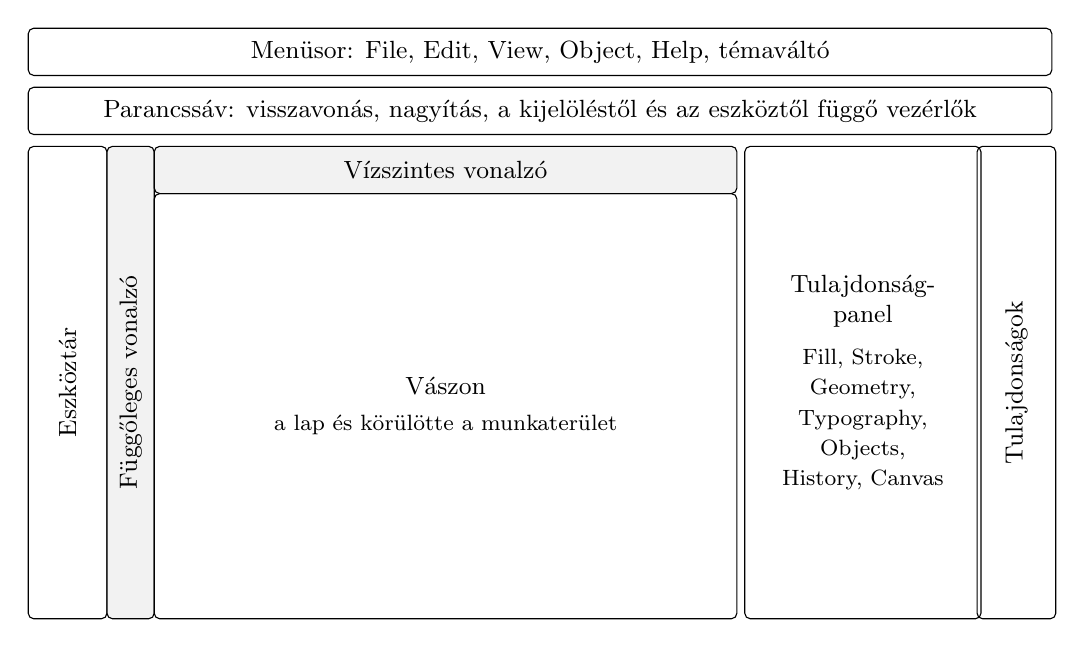
\begin{tikzpicture}[
  box/.style={draw, rounded corners=2pt, align=center, font=\small, inner sep=3pt},
  x=1cm, y=1cm]
  \node[box, minimum width=13cm, minimum height=0.6cm] (menu) at (6.5,7.3) {Menüsor: File, Edit, View, Object, Help, témaváltó};
  \node[box, minimum width=13cm, minimum height=0.6cm] (cmd) at (6.5,6.55) {Parancssáv: visszavonás, nagyítás, a kijelöléstől és az eszköztől függő vezérlők};
  \node[box, minimum width=1cm, minimum height=6cm] (tools) at (0.5,3.1) {\rotatebox{90}{Eszköztár}};
  \node[box, minimum width=0.6cm, minimum height=6cm, fill=black!5] (rulerv) at (1.3,3.1) {\rotatebox{90}{Függőleges vonalzó}};
  \node[box, minimum width=7.4cm, minimum height=0.6cm, fill=black!5] (rulerh) at (5.3,5.8) {Vízszintes vonalzó};
  \node[box, minimum width=7.4cm, minimum height=5.4cm] (canvas) at (5.3,2.8) {Vászon\\[2pt]\footnotesize a lap és körülötte a munkaterület};
  \node[box, minimum width=3cm, minimum height=6cm] (panel) at (10.6,3.1) {Tulajdonság-\\panel\\[4pt]\footnotesize Fill, Stroke,\\\footnotesize Geometry,\\\footnotesize Typography,\\\footnotesize Objects,\\\footnotesize History, Canvas};
  \node[box, minimum width=1cm, minimum height=6cm] (tabs) at (12.55,3.1) {\rotatebox{90}{Tulajdonságok}};
\end{tikzpicture}
\caption{A felület elrendezése asztali kijelzőn}
\label{fig:layout}
\end{figure}

A menüsor a ritkábban használt, de mindig elérhető parancsokat gyűjti össze: a fájlkezelést, a szerkesztési műveleteket, a nézet beállításait, az objektumokra vonatkozó műveleteket és a súgót. A parancssáv bal szélén mindig ott van a visszavonás, a megismétlés és a nagyítás, a többi vezérlője az aktuális eszköztől és a kijelöléstől függ. Egy kijelölt alakzatnál a forgatás, az átlátszóság és a tükrözés jelenik meg, több alakzatnál az igazítás és a logikai műveletek, a tollnál pedig egy rövid útmutató a használatához.

A bal oldali eszköztár tizenhárom eszköze hat csoportot alkot. Az első a kijelölés és a csomópontok szerkesztése, a második a vonalak és görbék rajzolása, a harmadik a zárt alakzatoké. Ezt követi a szöveg, majd a meglévő alakzatokon dolgozó foltecset és olló, végül a nézet mozgatása. Minden eszköznek saját billentyűje van, ezeket a súgó is felsorolja.

A jobb oldali tulajdonságsáv hét panelt nyit meg. A kitöltés és a körvonal panel a színeket és a vonal stílusát állítja. A geometria panelen a pozíció, a méret, a forgatás és a forgatási középpont adható meg, a tipográfia panelen a szöveg beállításai. Az objektumok panel a dokumentum fáját mutatja, az előzmények panel a visszavonható lépéseket, a vászon panel a lap méretét, hátterét, a rácsot és az illesztést. A panel szélessége húzással állítható, a nyitott panel fülére újra kattintva pedig a panel bezárul, és a vászon a teljes szélességet megkapja.

Keskeny kijelzőn a panel már nem férne el a rajz mellett. Ilyenkor a vászon alatt, alulról nyíló lapként jelenik meg, amelynek magassága a felső szélénél húzva állítható. Az eszköztár és a tulajdonságsáv a helyén marad, így nyitott panel mellett is elérhetők.

A műveletek többféle úton érhetők el, de egyik sem csak rejtett úton. A gyakoriak a parancssávban vannak, a helyzethez kötöttek a jobb gombbal vagy hosszú érintéssel nyíló helyi menüben, és a menüsor mindegyiket tartalmazza. A helyi menü csak az adott helyzetben végrehajtható műveleteket sorolja fel, mert a letiltott menüpontok nehezebben áttekinthetővé tennék.

\section{Technológiai választások}
\label{sec:technologies}

Az alkalmazás teljes egészében kliensoldali webalkalmazás, a technológiák kiválasztásakor ezért a böngészőben futó, szerver nélkül is használható megoldásokat kerestem. Ez a szakasz a keretrendszert, a fejlesztői eszközöket és a külső könyvtárakat mutatja be, \aref{tab:versions}. táblázat pedig a pontos verziókat is rögzíti.

\subsection{Svelte és TypeScript}

A Svelte komponensei egyetlen fájlban írják le a szerkezetet, a stílust és a viselkedést, a fordító pedig ezekből a DOM-ot közvetlenül módosító JavaScript kódot állít elő~\cite{svelte-overview}. Az alkalmazás állapotát Svelte \textit{store}-ok tárolják. A store olyan objektum, amelyre a komponensek feliratkozhatnak, és amely minden változásról értesíti őket~\cite{svelte-stores}. A származtatott store más store-ok értékéből számol, és csak akkor frissül, ha a forrása megváltozott. Egy szerkesztőben ugyanazt a dokumentumot a vászon, a panelek és az objektumlista egyszerre jeleníti meg, és ez a modell mindhármat automatikusan naprakészen tartja.

Általános komponenskönyvtárat, például a Bootstrapet, nem használtam. A szerkesztő vezérlői, a színválasztó, a csúszkák, a fogantyúk és az objektumlista, egyedi elemek, egy komponenskönyvtár pedig saját megjelenést és elrendezési szabályokat hozott volna, amelyek a sűrű szerkesztőfelülethez kevéssé illeszkednek.

A TypeScript használatát az adatmodell indokolja. Az alakzatok típusa egy közös típusmező szerint elágazó unió, angol nevén \textit{discriminated union}, és a típusellenőrzés segít észrevenni, ha egy függvény valamelyik alakzattípus kezelését kihagyja.

\subsection{Fejlesztői eszközök}

A projekt a Vite fejlesztői környezetet használja. Fejlesztés közben a Vite a forrásfájlokat natív ES modulokként szolgálja ki, ezért egy módosítás után elég az érintett modult újratölteni~\cite{vite}. Az éles változatot is a Vite csomagolja statikus fájlokká, amelyeket bármely webszerver kiszolgálhat.

A tesztek a Vitest keretrendszerrel futnak, amely a Vite beállításait használja, a komponensek teszteléséhez pedig a jsdom könyvtár ad böngészőszerű környezetet Node.js alatt~\cite{vitest,jsdom}. A böngészőben végzett ellenőrzések egy részét a Playwright eszközzel automatizáltam, amely programból vezérel egy Chromium böngészőt~\cite{playwright}.

\subsection{Geometriai és betűtípus-könyvtárak}

A geometriai algoritmusok többsége saját kód, három területen azonban külső könyvtárra támaszkodik a szerkesztő: a logikai műveleteknél és a vágásnál a paper.js, a körvonal útvonallá alakításánál és a foltecsetnél a Clipper, a szöveg útvonallá alakításánál pedig a fontkit könyvtárra. \Aref{tab:versions}. táblázat a fejlesztői eszközökkel együtt sorolja fel őket.

\begin{table}[!ht]
\caption{A felhasznált eszközök és könyvtárak}
\label{tab:versions}
\centering
\footnotesize
\begin{tabular}{|l|l|>{\raggedright\arraybackslash}p{0.55\textwidth}|}
\hline
\textbf{Név} & \textbf{Verzió} & \textbf{Szerep} \\ \hline
Svelte & 5.57.2 & felhasználói felület, állapotkezelés \\ \hline
TypeScript & 5.9.3 & programozási nyelv \\ \hline
Vite & 7.3.7 & fejlesztői szerver, éles változat csomagolása \\ \hline
Vitest & 3.2.7 & automatikus tesztek \\ \hline
jsdom & 26.1.0 & böngészőszerű környezet a tesztekhez \\ \hline
paper.js & 0.17.0 & logikai műveletek, alakzatok vágása \\ \hline
clipper-lib & 6.4.2 & körvonal útvonallá alakítása, foltecset \\ \hline
fontkit & 2.0.4 & szöveg útvonallá alakítása, OpenType-szövegszedés \\ \hline
woff2-encoder & 2.0.0 & WOFF2 betűtípusfájlok kibontása a fontkit számára \\ \hline
\end{tabular}
\end{table}

A sokszögek logikai műveleteire több klasszikus algoritmus ismert. Vatti söprővonalas algoritmusa tetszőleges, akár önmagukat metsző sokszögeket is kezel~\cite{vatti1992}, ennek továbbfejlesztése a Clipper könyvtár~\cite{clipper}. A Martínez-Rueda-Feito algoritmus $O((n+k)\log n)$ időben dolgozik, ahol $n$ a csúcsok, $k$ a metszéspontok száma~\cite{martinez2009}, ezt valósítja meg a polygon-clipping könyvtár~\cite{polygon-clipping}. A logikai műveletekhez a polygon-clipping és a clipper2-ts könyvtárat is megvizsgáltam. Mindkettő sokszögekkel dolgozik, a görbéket előbb rövid egyenes szakaszokra bontják. Két kör egyesítéséből így több száz sarokpontú alakzat lenne, amely kézzel már alig szerkeszthető. A paper.js a görbék metszéspontjait számolja ki, és az eredményt is görbékből építi fel~\cite{paperjs}. A körvonal útvonallá alakítása és a foltecset eredménye eleve sokszög, ezekhez a Clipper eltolási és egyesítési műveleteit használtam~\cite{clipper}.

\newpage

\section{Az alkalmazás rétegei}
\label{sec:architecture}

Az alkalmazás négy rétegből áll, ezeket és a köztük haladó adatfolyamot \aref{fig:architecture}. ábra mutatja.

\begin{figure}[!ht]
\centering
\begin{tikzpicture}[
  layer/.style={draw, rounded corners=2pt, align=center, font=\small, minimum height=0.9cm, inner sep=4pt},
  arr/.style={-{Stealth[length=2mm]}, thick},
  node distance=0.7cm and 0.8cm]
  \node[layer, minimum width=4.2cm] (ui) {Komponensek\\\footnotesize panelek, menük, parancssáv};
  \node[layer, minimum width=4.2cm, right=1.2cm of ui] (canvas) {Vászon (\texttt{Canvas.svelte})\\\footnotesize DOM-események};
  \node[layer, minimum width=4.2cm, below=of canvas] (tools) {Eszközök (\texttt{tools/})\\\footnotesize \texttt{PointerInfo} feldolgozása};
  \node[layer, minimum width=9.6cm, below=2.4cm of $(ui)!0.5!(canvas)$] (editor) {Szerkesztési műveletek (\texttt{stores/editor.ts})};
  \node[layer, minimum width=9.6cm, below=of editor] (stores) {Állapot: dokumentum és előzmények, felület, nézet, ideiglenes elemek (\texttt{stores/})};
  \node[layer, minimum width=9.6cm, below=of stores, fill=black!5] (utils) {Modell és tiszta függvények: alakzatok, útvonalak, SVG be- és kimenet (\texttt{utils/})};
  \draw[arr] (canvas) -- (tools);
  \draw[arr] (ui.south) -- (ui.south |- editor.north);
  \draw[arr] (tools.south) -- (tools.south |- editor.north);
  \draw[arr] (editor) -- (stores);
  \draw[arr, dashed] (stores.west) -- ++(-0.35,0) |- (ui.west);
\end{tikzpicture}
\caption{Az alkalmazás rétegei és az adatfolyam iránya; a szaggatott nyíl a store-ok értesítéseit jelöli}
\label{fig:architecture}
\end{figure}

A legalsó réteg az \texttt{utils} mappa. Itt van a dokumentum típusainak leírása és a mellékhatás nélküli, úgynevezett tiszta függvények: a határoló téglalapok számítása, az alakzatok mozgatása és méretezése, az útvonalak feldolgozása, az SVG importálása és előállítása. Ezek a függvények sosem módosítják a kapott alakzatot, hanem új alakzatot adnak vissza. Fölöttük a \texttt{stores} mappa store-jai tárolják a dokumentumot és az előzményeit, a felület állapotát a kijelöléssel és az aktuális eszközzel, a nézet nagyítását és eltolását, valamint az ideiglenes rajzelemeket, például a rajzolás közbeni előnézetet.

A dokumentumot csak az \texttt{editor} objektum műveletei módosítják. Ilyen az alakzat hozzáadása, a stílus módosítása, a csoportosítás, az igazítás, a logikai művelet és a beillesztés, és mindegyik egy elnevezett, visszavonható lépést hoz létre. A legfelső rétegben a rajzoló eszközök a vászontól kapják a mutató eseményeit, a komponensek pedig a felhasználó kattintásait. Mindkettő csak az \texttt{editor} műveleteit hívja, az eredményt pedig a store-okból olvassa vissza.

Ennek az egyirányú adatfolyamnak két haszna van. Egy művelet ugyanúgy viselkedik, akár a panelről, akár a menüből, akár a helyi menüből indítják. Az eszközök és a műveletek emellett böngésző nélkül is tesztelhetők, mert egy eszköz kipróbálásához elég mesterséges mutatóeseményeket átadni neki, majd megvizsgálni a dokumentumot.

\Aref{fig:move-sequence}. ábra ezt az adatfolyamot egy alakzat húzással történő mozgatásán mutatja be. A kijelölő eszköz a lenyomáskor előnézeti módba kapcsolja a dokumentumot, mozgatás közben csak az előnézetet frissíti, a felengedéskor pedig egyetlen elnevezett lépésként rögzíti a változást. A vászon a store-ra feliratkozva értesül minden módosításról, és ennek hatására rajzolja újra az alakzatokat.

\begin{figure}[!htbp]
\centering
\begin{tikzpicture}[
  font=\footnotesize,
  head/.style={draw, rounded corners=2pt, fill=black!5, minimum width=2.5cm, minimum height=0.7cm, align=center},
  msg/.style={-{Stealth[length=1.8mm]}},
  ret/.style={-{Stealth[length=1.8mm]}, dashed},
  lbl/.style={above, inner sep=1.5pt, font=\scriptsize},
  note/.style={font=\scriptsize, align=left, anchor=west}]
  \foreach \x/\n/\t in {0/c/{Vászon}, 2.95/t/{Kijelölő eszköz}, 5.9/e/{\texttt{editor}}, 8.85/d/{\texttt{documentStore}}, 11.8/r/{\texttt{ShapeRenderer}}} {
    \node[head] (\n) at (\x,0) {\t};
    \draw[black!45] (\n.south) -- (\x,-9.3);
  }
  % lenyomás
  \node[font=\scriptsize, align=right, anchor=east] at (-0.1,-1.3) {lenyomás};
  \draw[msg] (0,-1.3) -- node[lbl] {\texttt{down(info)}} (2.95,-1.3);
  \draw[msg] (2.95,-1.75) -- node[lbl] {\texttt{beginDrag()}} (5.9,-1.75);
  \draw[msg] (5.9,-2.2) -- node[lbl] {\texttt{beginPreview()}} (8.85,-2.2);
  \node[note] at (8.9,-2.55) {a kiinduló állapot\\megjegyzése};
  % mozgatás ciklus
  \draw[black!60, rounded corners=1pt] (-1.55,-3.2) rectangle (13.15,-6.55);
  \node[anchor=north west, font=\scriptsize\itshape, inner sep=2pt] at (-1.55,-3.2) {ismétlődik};
  \node[font=\scriptsize, align=right, anchor=east] at (-0.1,-4.0) {mozgatás};
  \draw[msg] (0,-4.0) -- node[lbl] {\texttt{move(info)}} (2.95,-4.0);
  \draw[msg] (2.95,-4.45) -- node[lbl] {\texttt{previewShapes(\dots)}} (5.9,-4.45);
  \draw[msg] (5.9,-4.9) -- node[lbl] {\texttt{preview(\dots)}} (8.85,-4.9);
  \draw[ret] (8.85,-5.45) -- node[lbl] {értesítés} (0,-5.45);
  \draw[msg] (0,-6.05) -- node[lbl] {módosított alakzatok} (11.8,-6.05);
  % felengedés
  \node[font=\scriptsize, align=right, anchor=east] at (-0.1,-7.2) {felengedés};
  \draw[msg] (0,-7.2) -- node[lbl] {\texttt{up(info)}} (2.95,-7.2);
  \draw[msg] (2.95,-7.65) -- node[lbl] {\texttt{commitDrag('Move')}} (5.9,-7.65);
  \draw[msg] (5.9,-8.1) -- node[lbl] {\texttt{commitPreview(\dots)}} (8.85,-8.1);
  \node[note] at (8.9,-8.45) {új bejegyzés\\az előzményekben};
  \draw[ret] (8.85,-9.0) -- node[lbl] {értesítés} (0,-9.0);
\end{tikzpicture}
\caption{Egy alakzat mozgatásának lépései a rétegeken át; a szaggatott nyilak a store értesítéseit jelölik}
\label{fig:move-sequence}
\end{figure}

\section{Adatmodell}
\label{sec:data_model}

A dokumentum JSON formában tárolható adatszerkezet. Az alakzatok fáján kívül a lap méretét, a hátteret, egy opcionális háttérképet és a vonalzókból húzott segédvonalakat tartalmazza. Az alakzatok típusát a \texttt{type} mező adja meg, és ez dönti el, milyen geometriai adatok tartoznak hozzájuk. \Aref{tab:shape-types}. táblázat az alakzattípusokat és a kimenetben nekik megfelelő SVG-elemeket mutatja.

\begin{table}[!htbp]
\caption{Az alakzattípusok, geometriai adataik és SVG megfelelőjük}
\label{tab:shape-types}
\centering
\footnotesize
\begin{tabular}{|l|>{\raggedright\arraybackslash}p{0.5\textwidth}|l|}
\hline
\textbf{Típus} & \textbf{Geometria} & \textbf{SVG-elem} \\ \hline
\texttt{rectangle} & bal felső sarok, szélesség, magasság, saroksugarak & \texttt{<rect>} \\ \hline
\texttt{ellipse} & középpont, két sugár & \texttt{<ellipse>} \\ \hline
\texttt{line} & két végpont & \texttt{<line>} \\ \hline
\texttt{path} & csomópontok be- és kimenő fogantyúval, zártság, kitöltési szabály & \texttt{<path>} \\ \hline
\texttt{text} & kezdőpont, sorok, betűtípus, díszítővonalak, térközök & \texttt{<text>} \\ \hline
\texttt{image} & bal felső sarok, méret, a kép \texttt{data:} URL-je & \texttt{<image>} \\ \hline
\texttt{group} & a csoport tagjai & \texttt{<g>} \\ \hline
\end{tabular}
\end{table}

Az alakzatok közös adatai az egyedi azonosító, név, láthatóság, zárolás, átlátszóság, kitöltés, körvonal és vonalvastagság, vonalvég, sarok, szaggatási minta és forgatás.

\paragraph{Útvonalak.} A szerkesztő az útvonalat csomópontok listájaként tárolja, az SVG \texttt{d} attribútumának parancsait csak importáláskor és exportáláskor használja. Egy csomópontnak van helye, opcionális bejövő és kimenő fogantyúja, és egy jelzője arról, hogy sima-e. Két csomópont között egyenes szakasz van, ha a köztük lévő oldalon egyiknek sincs fogantyúja, különben harmadfokú Bézier-görbe. Ebben a formában minden csomópont és fogantyú közvetlenül megfogható. Az SVG másodfokú görbéit és íveit az importáló harmadfokú görbékké alakítja.

\paragraph{Színek és színátmenetek.} A kitöltés és a körvonal értéke egy karakterlánc. Lehet \texttt{none}, egy \texttt{\#rrggbb} színkód vagy átlátszósággal együtt \texttt{\#rrggbbaa}, illetve egy színátmenet leírása. Egy lineáris átmenet például \texttt{lg:90;\#1e3c72@0,\#f7b267@100} alakú. Az első szám a szög fokban, utána a színek következnek a helyükkel együtt, százalékban. A színek és a színátmenetek így ugyanazon a kódon haladnak át stílus másolásakor, összehasonlításkor vagy visszavonáskor. Ha a színátmenet külön objektum lenne, ezeket a műveleteket két változatban kellene megírni. Exportáláskor minden színátmenet egy \texttt{<defs>} elembe kerül, és az alakzat \texttt{url()} hivatkozással használja.

\paragraph{Csoportok.} A csoport forgatása és átlátszósága a csoport egészére vonatkozik, a tagok koordinátái pedig úgy értendők, mintha a csoport nem lenne elforgatva. A felhasználó beléphet egy csoportba, ekkor a kijelölés és a szerkesztés a csoport tagjaira vonatkozik.

\paragraph{Forgatás és forgatási középpont.} Az alakzat forgatása fokban, a saját, el nem forgatott határoló téglalapjának közepe körül értendő, az exportált fájlban ebből lesz a \texttt{rotate(szög cx cy)} transzformáció. Ehhez járul egy opcionális forgatási középpont, amely a határoló téglalaphoz viszonyított arányként adja meg, mely pont körül forog az alakzat a szerkesztőben. A forgatási középpont csak szerkesztési segédlet. Forgatáskor a szerkesztő a szöget és a pozíciót együtt módosítja úgy, hogy a kijelölt pont a helyén maradjon, a tárolt forgatás pedig mindig a téglalap közepe körüli marad. Erre a feltevésre épül a határoló téglalap, a méretezés, a tükrözés és az export minden számítása, egy valódi, tetszőleges forgatási középpont mindegyiket bonyolultabbá tenné.

\section{Az előzmények kezelése}
\label{sec:history_design}

A visszavonásra két elterjedt tervezési minta létezik~\cite{gof}. A \textit{Command} minta minden műveletet olyan objektumként tárol, amely a végrehajtást és a visszacsinálást is ismeri. Berlage ezt a megoldást grafikus felületekre a tetszőleges korábbi lépés visszavonásáig, a szelektív visszavonásig fejlesztette tovább~\cite{berlage1994}. A \textit{Memento} minta ehelyett az állapotról készít pillanatképet. A szerkesztő a második megoldást követi. A dokumentum adatai sosem módosulnak helyben, minden művelet új dokumentumot készít, amely a változatlan alakzatokat megosztja az előzővel. Egy pillanatkép ezért csak a megváltozott alakzatok helyét foglalja, a visszavonás pedig egyetlen hivatkozás cseréje. Ez a perzisztens adatszerkezetek elve, amelyekben a módosítás új változatot hoz létre, a régi változatok elérhetők maradnak, és a változatok a közös részeiket megosztják~\cite{driscoll1989,okasaki1998}. A legfontosabb előnye, hogy egy új művelethez nem kell külön visszacsináló kódot írni, és így ilyen kód hibájából sem állhat vissza rossz állapot.

Az előzmények a korábbi állapotokból, a jelenlegi állapotból és a visszavont, de megismételhető állapotokból álló idővonalat alkotnak. Minden bejegyzés a nevében szereplő művelet utáni állapotot tárolja. Az előzmények panelen egy bejegyzésre kattintva tehát pontosan az a rajz jelenik meg, amelyet a bejegyzés neve leír. Egy új művelet törli a megismételhető állapotokat, és a szerkesztő legfeljebb kétszáz lépést őriz meg.

Egy felhasználói művelet néha sok egymás utáni módosításból áll. Egy szín csúszkával történő állítása vagy egy szám begépelése egy közös összevonási kulccsal érkezik, és a rövid időn belül egymást követő módosítások egyetlen bejegyzésbe olvadnak. A vásznon végzett húzás közben, például egy alakzat mozgatásakor, csak egy előnézet változik, és az előzményekbe csak a felengedéskor kerül egy lépés. Ha a húzás végül semmit sem változtatott, bejegyzés sem keletkezik.

\section{Az eszközök közös felülete}
\label{sec:tool_design}

Minden eszköz ugyanazt a felületet valósítja meg, amelyet \aref{lst:tool}. programkód mutat. A vászon a böngésző mutatóeseményeit dokumentumkoordinátákká alakítja, közben figyelembe veszi a nagyítást, a belépett csoportot és az illesztést, majd az aktuális eszköznek adja tovább. A \texttt{target} mezőből az eszköz azt is megtudja, mi van a mutató alatt.

\begin{lstlisting}[style=TS, caption={Az eszközök közös felülete (\texttt{tools/types.ts}, rövidítve)}, label=lst:tool]
interface PointerInfo {
  p: Point;          // document coordinates, snapped
  raw: Point;        // document coordinates, never snapped
  shift: boolean; alt: boolean; ctrl: boolean;
  target: Element | null;   // the element under the pointer
}
interface Tool {
  down(i: PointerInfo): void;
  move(i: PointerInfo): void;
  up(i: PointerInfo): void;
  dblclick?(i: PointerInfo): void;
  key?(e: KeyEvent): boolean;  // true: the key was consumed
  escape(): boolean;           // false: the canvas deselects
  deactivate(): void;          // finish or discard pending work
  busy(): boolean;
}
\end{lstlisting}

Az eszközök nem érik el közvetlenül a DOM-ot. Rajzolás közben az előnézetet és a segédvonalakat egy ideiglenes store-ba írják, amelyet a vászon jelenít meg, a kész alakzatot pedig az \texttt{editor} műveleteivel adják a dokumentumhoz. Az eszközök nevét, ikonját és billentyűjét egyetlen katalógus tartalmazza, ebből dolgozik az eszköztár és a súgó is, ezért a kettő nem térhet el egymástól.

A toll és a körív eszköz egy közös, éppen rajzolt útvonalon dolgozik. Rajzolás közben a B és az A billentyűvel váltva ugyanaz az útvonal folytatódik, és egy alakzaton belül egyenes szakaszok, Bézier-görbék és körívek követhetik egymást. Ugyanez a közös útvonal teszi lehetővé, hogy egy kijelölt nyitott útvonal végpontjáról indított rajzolás azt az útvonalat folytassa.

\section{Tárolás és fájlformátumok}
\label{sec:storage_design}

A szerkesztő a rajzot, a beállításokat és az exportált fájlokat külön kezeli. A rajz projektfájlba menthető, amely egy formátumazonosítót, egy verziószámot és magát a dokumentumot tartalmazó JSON-dokumentum. Az SVG csak saját kiterjesztésekkel őrizhetné meg mindazt, amire a szerkesztőnek szüksége van, például az alakzatok zárolását, a segédvonalakat vagy a forgatási középpontokat. Az automatikus mentés ugyanezt a formátumot írja a böngésző helyi tárolójába.

A rács, az illesztés, a panelek mérete és a hasonló beállítások azt írják le, hogyan dolgozik a felhasználó, és nem azt, amit rajzolt. Ezek ezért a böngésző helyi tárolójába kerülnek, és egy projektfájl bárhol megnyitva ugyanúgy néz ki. Kivételt a segédvonalak jelentenek, mert azok egy adott rajzhoz tartoznak, ezért a projektfájlba kerülnek. Az exportált SVG szabványos, a szerkesztő saját adatai nem szerepelnek benne. A raszteres képek az exportált SVG-ből készülnek, amelyet a szerkesztő a böngésző vásznára rajzol.

A böngésző helyi tárolójának mérete eredetenként korlátozott~\cite{whatwg-webstorage,mdn-storage}, egy nagy beágyazott képet tartalmazó rajz el is érheti ezt a korlátot. Ha az automatikus mentés nem sikerül, a szerkesztő figyelmeztet, és a projektfájlba mentés továbbra is elérhető.
